\documentclass{article}
\usepackage[english]{babel}
\usepackage{graphicx}
\graphicspath{{Images/}}
\usepackage{geometry}
\geometry{a4paper, top=2cm, bottom=2cm, left=1.0cm, right=1.0cm}
\usepackage{amsthm}
\usepackage{amsmath}
\usepackage{fixltx2e}
\usepackage{amsfonts}
\usepackage{xcolor}
\usepackage{verbatim}
\usepackage{amssymb}
\newtheorem{theorem}{\textbf{Teorema}}
\newtheorem{corollary}{\textbf{Corollario}}
\theoremstyle{definition}
\newtheorem{definition}{\textbf{Definizione}}

\title{Toeria della regolazione}
\author{Lorenzo Rossi}
\begin{document}
\maketitle
Nella teoria della regolazione consideriamo un sistema lineare affetto da disturbi e tale che la sua uscita deve inseguire asintoticamente un segnale di riferimento noto.
\begin{equation*}
	\Sigma:\begin{cases}
		\dot{x}=Ax+Bu+Pd \\
		e=Cx+Qd
	\end{cases}
\end{equation*}
con \(x(t)\in\mathbb{R}^{n},u(t)\in\mathbb{R}^{m},e(t)\in\mathbb{R}^{p},d(t)\in\mathbb{R}^{r}\) e le matrici \(A\in\mathbb{R}^{n\times n},B\in\mathbb{R}^{n\times m},P\in\mathbb{R}^{n\times p},C\in\mathbb{R}^{p\times n},Q\in\mathbb{R}^{p\times r}\) note e costanti.\newline
In questo sistema si identifica:
\begin{itemize}
	\item \(d(t)\) che rappresenza un segnale esogeno composto da una componente del disturbo associato al processo e una componente dei segnali di riferimento. La sua dinamica è descritta da un sistema lineare:\begin{equation*}
		      \Sigma_{d}=S d\quad S\in\mathbb{R}^{r\times r},d(t)=\begin{bmatrix}
			      w(t) \\r(t)
		      \end{bmatrix}\in\mathbb{R}^{r}
	      \end{equation*}
	\item \(e(t)\) è l'errore di inseguimento del comportamento del sistema rispetto al comportamento ideale. Di norma vogliamo che si raggiunga l'obiettivo di \textbf{regolazione a zero}: l'errore deve convergere a zero tramite un controllo \(u(t)\) opportuno. Inoltre, la specifica di regolazione a zero implica che i disturbi non influenzano il comportamento del sistema e l'uscita \(y=Cx(t)\) insegue asintoticamente il segnale di riferimento \(r(t)=-Q d(t)\)
\end{itemize}
Il controllore \(u(t)\) necessario per la regolazione a zero può essere ottenuto in due modi:
\begin{itemize}
	\item \textbf{Controllore statico in feedback dallo stato \(x(t)\)}: Supponiamo che \(x(t)\) sia lo stato e \(d(t)\) sia il segnale esogeno, entrambi misurati. Allora si progetta la legge di controllo \(u=K x+L d\)
	      \begin{figure}[h]
		      \centering
		      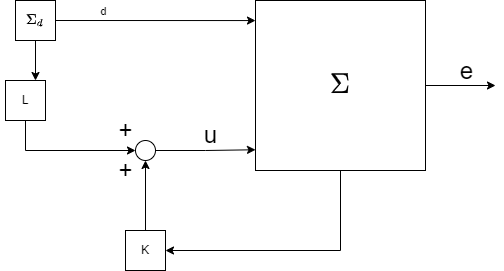
\includegraphics[scale=0.3]{uStatico.drawio.png}
	      \end{figure}
	\item \textbf{Controllore dinamico dall'errore \(e(t)\)}: questo controllore non necessita che i segnali \(x(t),d(t)\) siano misurati, ma si costruisce un osservatore la cui uscita viene utilizzata per progettare un controllo \(u(t)\).\begin{equation*}
		      \begin{cases}
			      \dot{\chi}= F\chi+G e \\
			      u=H\chi
		      \end{cases}
		      \quad F\in\mathbb{R}^{\nu\times\nu},G\in\mathbb{R}^{\nu\times\nu}\text{note e costanti}
	      \end{equation*}
          \begin{figure}[h]
            \centering
            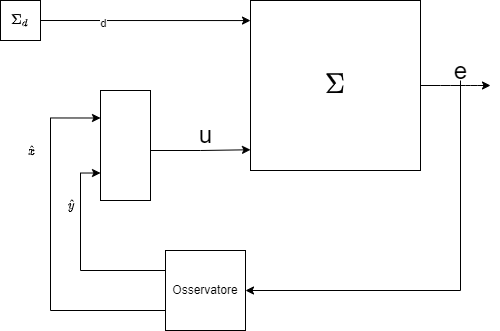
\includegraphics[scale=0.3]{uDynamic.drawio.png}
        \end{figure}
\end{itemize}
Nella teoria di regolazione ci si riferisce principalemnte a due tipi di problemi.
\begin{definition}{\textbf{Problema di regolazione a full information}}\\
	Considerato il sistema:\(\begin{cases}
		\dot{x}=Ax+Bu+Pd \\
		e=Cx+d
	\end{cases}\) affetto da disturbi generati dall'esosistema \(\dot{d}=Sd\) interconnesso con il controllore \(u=K x+L d\). Il \textbf{problema di regolazione a informazione completta} è quello di determinare le matrici \(K,L\) dek controllore tali che siano soddisfatte:
    \begin{itemize}
		\item \textbf{\emph{Stabilità} (S)}:Il sistema \(\dot{x}=(A+BK)x\) sia asintoticamente stabile;
		\item \textbf{\emph{Regolazione} (R)}: tutte le traiettorie del sistema \(\begin{cases}
			      \dot{d}=Sd              \\
			      \dot{x}=(A+BK)x+(BL+O)d \\
			      e=Cx+QD
		      \end{cases}\) siano tali che \(\lim_{t\rightarrow\infty}e(t)=0\)
	\end{itemize}
\end{definition}
\begin{definition}{\textbf{Problema di regolazione con retroazione dall'errore}}\\
    Considerato il sistema:\(\begin{cases}
		\dot{x}=Ax+Bu+Pd \\
		e=Cx+d
	\end{cases}\) affetto da disturbi generati dall'esosistema \(\dot{d}=Sd\) interconnesso con il controllore \(\begin{cases}
        \dot{\chi}=F\chi + Ge\\
        u=H\chi
    \end{cases}\). Il \textbf{problema di regolazione in feedback dall'errore} è il problema di determinare le matrici \(F,G,H\) del controllore tali che siano soddisfatte:
    \begin{itemize}
        \item \textbf{\emph{Stabilità} (S)}: Il sistema \(\begin{cases}
            \dot{x}=Ax+BH\chi \\
            \dot{\chi}=F\chi+GC\chi
        \end{cases}\) sia asintoticamente stabile;
        \item \textbf{\emph{Regolazione} (R)}: tutte le traiettorie del sistema \(\begin{cases}
            \dot{d}=Sd\\
            \dot{x}=Ax+BH\chi+Pd \\
            \dot{\chi}=F\chi+G(Cx+Qd)\\
            e=Cx+Qd
        \end{cases}\) siano tali che  \(\lim_{t\rightarrow\infty}e(t)=0\).
    \end{itemize}
\end{definition}
\section*{Problema di regolazione a Full Information}
Per poter risolvere il problema di regolazione a full information dobbiamo fefinire le seguenti ipotesi strutturali:\begin{itemize}
    \item Sia \(S\) la matrice dell'esosistema e \(\lambda\in\sigma{(S)}\), allora \(\forall\lambda\in\sigma{(S)},Re(\lambda)\geq 0\): ciò implica che \(\nexists d(0) \) tale che \(d(t)\) converge asintoticamente a zero. Se così non fosse \(d(t)\) non influisce sul comportamento asintotico del sistema e quindi basterebbe solamente stabilizzare il sistema per raggiungere l'obbiettico;
    \item Il sistema \(\dot{d}=Sd\) con \(d=0\) è raggiungibile: ciò implica che è possibile assegnare arbitrariamente gli autovalori di \(A+BK\)
\end{itemize}
\begin{theorem}
    Considerato il problema di regolazione a full information, supponiamo che \(\forall\lambda\in\sigma{(S)}:Re(\lambda)\geq 0\) e che \(\exists K,L\) tali che il sistema \(\dot{x}=(A+BK)x\) sia asintoticamente stabile, allora la condizione di regolazione è soddisfatta se e solo se \(\exists \Pi\in\mathbb{R}^{n\times r}\) tali che soddisfano le equazioni\begin{equation*}
        \begin{cases}
            \Pi S=(A+BK)\Pi+(P+BL)\\
            0=C\Pi+Q
        \end{cases}
    \end{equation*}
\end{theorem}
\begin{corollary}{\textbf{Equazione di Sylvester}}\\
    Sia \(A\in\mathbb{C}^{m\times m},B\in\mathbb{C}^{n\times n},C\in\mathbb{C}^{m\times n}\), l'equazione di Sylvester è una equazione matriciale lineare nella forma \(AX+BX=C\) con \(X\in\mathbb{C}^{m\times n}\). Valgoono i seguenti enunciati:\begin{itemize}
        \item L'equazione di Sylvester ha soluzione se e solo se \(A\) e \(-B\) non hanno nessun autovalore in comune;
        \item L'equazione di Sylvester ha un'unica soluzione se \(A\) e \(-B\) non hanno autovalori in comune o un'unfinità di soluzioni composte da \(X=X_{0}+\hat{X}\) con \(X_{0}\) ottenuta da \(AX+XB=0\)
    \end{itemize}
    \begin{proof}{Equazione di Sylvester}
        Gli autovalori di \(G=(I_{n}\bigotimes A)+(B^{T}\bigotimes I_{n})\) sono \(\lambda_{A}+\lambda_{B},\forall \lambda_{A}\in\sigma{(A)},\lambda_{B}\in\sigma{(B)}\). Inoltre ha un'unica soluzione se G non è singolare e quindi se non esiste nessun autovalore \(\lambda_{G}=0\). Quindi:
        \begin{equation*}
            \lambda_{A}+\lambda_{B}\neq 0\rightarrow \lambda_{A}\neq-\lambda_{B}\rightarrow \lambda_{A}\neq\lambda_{B}\forall \lambda_{A}\in\sigma{A},\lambda_{B}\in\sigma{B}
        \end{equation*}
    \end{proof}
\end{corollary}
\begin{proof}{\textbf{Teorema Regolazione Full Information}}
    Consideriamo il sistema \(\begin{cases}
        \dot{d}=Sd              \\
        \dot{x}=(A+BK)x+(BL+O)d \\
        e=Cx+QD
    \end{cases}\) e il cambio di coordinate \(\hat{d}=d,\hat{x}=x-\Pi d\) con \(\Pi \) soluzione dell'equazione di Sylvester \( \begin{cases}
        \Pi S=(A+BK)\Pi+(P+BL)\\
        0=C\Pi+Q
    \end{cases}\).\newline
    Si nota che la soluzione è unica dato che:\begin{equation*}
        \begin{cases}
            \lambda\in\sigma{(A+BK)},Re(\lambda )< 0 \\
            \lambda\in\sigma{(S)},Re(\lambda )\geq 0
        \end{cases}\rightarrow\sigma{(A+BK)}\cap\sigma{(S)}=\{\varnothing \}\Rightarrow \forall(P+BL)\exists!\Pi
    \end{equation*}
    Riscrivendo il sistema nelle nuove coordinate:
    \begin{equation*}
        \begin{cases}
            \dot{\hat{x}}=\Pi S\dot{\hat{d}}=(A+BK)\hat{x}+(A+BK)\Pi\hat{d}+(BL+P)\hat{d}\\
            \hat{e}=C\hat{x}+C\Pi\hat{d}+Q\hat{d}\\
            \dot{\hat{d}}=S\hat{d}
        \end{cases}
        \rightarrow^{Dal teorema}\begin{cases}
            \dot{\hat{x}}=(A+BK)\hat{x}\\
            e=C\hat{x}+(C\Pi+Q)\hat{d}\\
            \dot{\hat{d}}=S\hat{d}
        \end{cases}
    \end{equation*}
    Dalla stabilità sappiamo che \(\lim_{t\rightarrow\infty} \hat{x}(t)=0\) e dalla regolazione \(\lim_{t\rightarrow\infty}e(t)=0\leftrightarrow C\Pi+Q=0\). Ciò implica che anche per osillazioni di \(d,x\), si regolarizza la soluzione vincolandola sulla bisettrice del piano \(x,d\).
\end{proof}

\end{document}